\chapter{Implementation} \label{cha:impl}

This section will focus on the implementation of the zero core \gls{ide}. In
section \ref{sec:stack}, we will mention technologies used, and why they were
chosen. In section \ref{sec:mod1} and \ref{sec:mod2}, we will discuss the
different iterations the application architecture had, and why they were subpar,
compared to section \ref{sec:mod3}, which is the implementation of the zero core
\gls{ide}. Section \ref{sec:testing} will explain the necessity of testing when
using such a modular design, and explore the ease of which functionality can be
tested.

\section{Tech Stack} \label{sec:stack}

A module can extend an application at either compile time, or during runtime.
This could be achieved by using an interpreted language like JavaScript or
Python. The issue with using a dynamically typed language like Python or
JavaScript, is that it enhances the risk for runtime issues occurring, and when
dealing with scenarios like writing to files, or running long processes like
compiling a program, it is important to avoid such issues. So using a typesafe
language, that can \textit{transform} runtime errors into compile time errors,
is preferred. Furthermore, being able to support runtime modules, in a language
agnostic manner, necessarily means that the core \gls{ide} needs good
\gls{abi} support, and therefore should be implemented in a low level language.
But what does \textit{low level} language mean? And what is an \gls{abi}?

\subsection{Low level languages}

Programming languages has changed over time. In the beginning, a program was a
series of ones and zeros, representing instructions a computer should do. Since
then, we have moved several abstraction layers above what is commonly referred
as \textit{bare metal} programming. From writing in hexadecimal instead of
binary, to machine instructions, to more generic programming language, like C.
What was different with C, compared to writing direct machine instructions, was
that an external program, a compiler, could translate C code to machine
instructions specific to the computers' \gls{cpu} architecture, this meant a
single program, written in C, could be compiled to many different computers. So,
at the time C came out, it was considered a \textit{high level} programming
language, because the language a developer was writing in, had a higher level of
abstraction. Today this notion of \textit{low} and \textit{high} level languages
has changed. A \textit{low level} language is close to how a \gls{cpu}
\textit{thinks}, which has traditionally meant that C is a low level programming
language, but some authors \cite{cNotLowLevel} argue that this is no longer the
case. In any case, we will use \textit{low level} to mean a programming
languages like C, where direct memory manipulations is a feature of the
language.

\subsection{Application Binary Interface (ABI)}

An \gls{abi} is an interface between two programs. This could be a
dynamic library used by a C program, where both binaries agree on how the data
is stored. The reason they need to agree on how data is ordered in the memory,
is that accessing into unowned memory could lead to \textit{undefined} behavior.

\paragraph{Undefined behavior} In programming, undefined behavior is behavior
that is not defined by the specification of the language being used.
\todo{Is this a correct explanation?}

\todo{Connect these two sections better}

\paragraph{Why not C?} C has good parts, like the C-\gls{abi}, which most
languages have bindings too. Using C would mean allowing those languages to
interface with our project, meaning, one step closer to a language agnostic
module architecture. But C has issues, like being the number one cause in
security issues. (This is just because so much of our infrastructure is written
in C, but y'know.) These security issues are mostly caused by memory management.
Would be cool if the C compiler could notify a developer if they were developing
something that could cause an issue in the future. Enter, Rust.
\todo{Rewrite this paragraph}

\subsection{Rust}

Rust is a general purpose programming language, designed for, amongst other
things, type safety, memory safety, and concurrency. When programming in Rust,
the bugs common in other languages, like null pointers, buffer overflow and data
races are detected at compile time. Most of these are features of Rusts
ownership rules. These rules, enforced by the compiler, ensure that values are
safely dropped, (freed), this ensures that all variables referenced in Rust have
a value, and can be safely evaluated. It works by simply dropping values when
they are out of scope. The example in listing \ref{lst:ownership}, the
\textbf{name} variable is declared, and used as an argument in the
\textbf{greeting} function. We cannot call the function again with
\textbf{name}, since at the end of \textbf{greeting}, before it returns,
\textbf{name} is dropped, since once we called \textbf{greeting}, the
\textbf{main} method no longer \textit{owned} \textbf{name}, as the ownership
was transferred to \textbf{greeting}. We could \textit{fix} this by changing the
argument type from \textit{name: String}, to \textit{name: \&String}, (commonly
written as \textit{name: \&str}), and adding the borrow symbol to the argument in
the method invocation, as shown in listing \ref{lst:ownership-ref}.

\begin{center}
  \lstinputlisting
    [ language=Rust
    , caption={Ownership example (Rust)}
    , label=lst:ownership
    ]{./code/rust-ownership.rs}
\end{center}

\begin{center}
  \lstinputlisting
    [ language=Rust
    , caption={Ownership example with reference (Rust)}
    , label=lst:ownership-ref
    ]{./code/rust-ownership-ref.rs}
\end{center}

This same principle ensure the other mentioned features of the language,
including performance, as with the borrow checker, there is no need for a
garbage collector. Another Rust feature are so-called \textit{macros}. A macro
is some code that is evaluated and executed at compile time, that may change
the source code. An example of this, can be seen in listing \ref{lst:ownership}.
The \textbf{println!} is a macro invocation. \textbf{println!} is used so that
the developer doesn't have to format the expressions being used, this is handled
by the macro. This is helpful because redundant work can be automated.

Furthermore, Rust has good cross-platform support, ensuring
we can write OS-agnostic code, and compile it to specific targets, without much
hassle. Since Rust is low-level, it has good bindings to C, ensuring
compatibility with future models, made in other languages, by use of the Rust
\gls{abi}.

\subsubsection{Rust Application Binary Interface}

\todo{rewrite}

Rusts \gls{abi} is not stable! Because it is not supported by their semantic
versioning. This means even a bug fix in the compiler, could break the
\gls{abi}. So if an application, written in Rust, is compiled in version 1.8.0,
if this application relies on a Rust library that is compiled in version 1.8.0,
everything is okay. But if the application is later recompiled with a compiler
in version 1.8.1, then \textit{undefined} behavior could occur. One of the ways
undefined behavior was avoided, was using the \textit{abi\_stable}-crate, which
enables \textit{safe} loading of external libraries, meaning modules. This is
only an issue for runtime modules, which means they need to be handled
differently than compile time modules.
\todo{Explain this more concretely}

If the types in the core application change, either by expansion or renaming or
such, the crate would crash the application during startup, because the existing
module would have a different expectation of what types existed, which again,
could lead to undefined behavior. But, this due to the implementation of a
runtime module using the \textit{abi\_stable}-crate, as one could design a
module to be expanded in the future, but due to the stability of the \gls{api},
this was deemed unnecessary.

\subsection{Tauri}

Tauri is a framework for Rust, which enables us to create a cross-platform
application. Any frontend framework that compiles to \gls{html}, JavaScript and
\gls{css} can be used as the \gls{gui}. Such a \gls{gui} is commonly referred to
as a \textit{web view}. This framework also adds support for invoking Rust
methods in the frontend framework, and vice-versa. This allows for support of
JavaScript modules, without much fuzz. Tauri archives with \gls{ipc}, which
allows for isolated processes to communicate securely. For JavaScript to Rust,
this is achieved with something called \textit{Commands}, which acts as an
abstraction on top of the \gls{ipc}, which turns the invocation to a
frontend-backend architecture.

\subsubsection{TypeScript}

Any frontend framework that compiles to \gls{html}, JavaScript and \gls{css} can
be used with Tauri, so TypeScript was chosen. TypeScript offers a lot of
features over JavaScript, amongst them being able to \textit{type} functions,
ensuring null/undefined-safety. Furthermore, by using crates like
\textit{ts-rs}, Rust types can be annotated with attribute macros, which create
a one-to-one mapping between the Rust type, and the serialized JSON object, to
be used in TypeScript, allowing for even more type safety, and ensuring that the
types used in the \gls{ide} only have to be defined one place.

Allowing for any JavaScript library to be used, enabled a low development time
of \gls{ui} components, since this is something that a lot of \gls{ui} and user
experience designers have looked into. So existing code for this already exists
and can be used. \gls{npm}, for example, is a package registry for JavaScript.
It contains around \textit{34 million} libraries, all of which are usable in
this architecture. If the functionality that these libraries are useful for the
application, is another question. This functionality allows for quick
development time for modules, which means features that are standard in
\gls{ide} can be quickly and easily added.

\subsection{Security}

This framework gives a lot of security which is needed in an
application which runs third party code.
\todo{Expand}
\todo{Look into isolation pattern from Tauri}

\subsubsection{Module Validation}

\todo{Mention module validation}

\todo{Also expand on the module-validation part, third-party-code, and all that.}

Before the finalization of this state representation, there was some
discussion, on how best to represent a number. Because, in JavaScript, there is
no distinction between a floating-point number, and a decimal number. This
\textit{leakage} was stopped by adding extra validation in the core, using the
\textit{io-fp} library, which validates data sent from a module, regardless if
its from the frontend or backend This will be discussed more in the next
section.

This lead to the development of two systems. \gls{rsms} and \gls{jsms}.
\todo{Mention in the next section how RSMS and JSMS are just backend frontend}
It was necessary to distinguish the different module systems, due to the way
they would be loaded by the core application.
\todo{Mention different methods of loading modules}
The \gls{rsms}, being written in Rust, meant it needed extra safeguards, as
loading of shared object files, during runtime, could lead to undefined
behavior.
\todo{Expand this point}

The \gls{jsms} is similar to the Rust example, except that the undefined
behavior, in this case, is exceptions being thrown. Since third party code is
being run, nothing can be trusted.
\todo{Mention this earlier}
All module invocations and outputs needs to be sanitized before it can be used
in the core application. This is achieved by wrapping all invocations in a
\textit{try-catch}, and using the \textit{io-fp} library to decode types during
runtime. This means that all modules in \gls{jsms} are actually of the type
shown in listing \ref{lst:jsmsModule}. Which using \textit{io-fp}, can be
handled as shown in listing \ref{lst:jsmsHandlingInit}. This
\lstinline[language=Haskell]{Either Error State} or
\lstinline[language=Haskell]{Either Error HTML} can be handled by other modules,
if there is a way to recover from the error. The \textit{standard} way for the
core to \textit{correct} this error, is to \textit{just} log the error. But this
turns an unrecoverable error into a recoverable one, given that it is an
acceptable result to \textit{ignore} the error.

\begin{center}
  \lstinputlisting
    [ language=TypeScript
    , caption={JSMS Module Type}
    , label=lst:jsmsModule
    ]{./code/jsms-example.ts}
\end{center}

\begin{center}
  \lstinputlisting
    [ language=TypeScript
    , caption={Module Module-Init Handling}
    , label=lst:jsmsHandlingInit
    ]{./code/jsms-handling-init.ts}
\end{center}

\begin{center}
  \lstinputlisting
    [ language=TypeScript
    , caption={Module Module-Update Handling}
    , label=lst:jsmsHandlingUpdate
    ]{./code/jsms-handling-update.ts}
\end{center}

\begin{center}
  \lstinputlisting
    [ language=TypeScript
    , caption={Module Module-View Handling}
    , label=lst:jsmsHandlingView
    ]{./code/jsms-handling-view.ts}
\end{center}

\todo{These are just put here, add some text explaining why}

\begin{center}
  \lstinputlisting
   [ language=Haskell
   , caption={Module Unverified Type}
   , label=lst:moduleTypeUnverified
   ]{./code/module-unverified-example.ts}
\end{center}

This architecture also has the issue about verification of modules, but only on
functions, as simple fields can be validated using the
\lstinline[language=JavaScript]{typeof} operator. It is possible to do
\textit{some} verification on functions in TypeScript, but this is only a) Is it
a function, and b) does it have the correct amount of arguments. In this case,
one. Nothing about the typing of the function can be ascertained at runtime,
without explicitly invoking the function.


\section{Module V.1} \label{sec:mod1}

We did not attempt at first, to create a zero core application; this was a
\textit{natural} conclusion to the existing problem. The first attempt was a
simple generic \gls{ide}, in which the module architecture was a concern from
day one of development. The general plan was this:

\begin{enumerate}
  \item Create an \gls{ide}
  \item Extend the \gls{ide}, to allow for a module architecture
  \item Modules call the application using some DSL
\end{enumerate}

Since any JavaScript frontend framework could be used, React was chosen, one of
the reason for this choice was due to its popularity, which again, would speed
up the development time of the application, but also due to the way React
renders. Between two different re-renders of the application, React can check
the difference between the \gls{vdom}, which is React's representation of the
\gls{dom}. It then only changes what is needed in the \gls{dom}, instead of
re-creating the entire \gls{dom}, which makes the render time quick.

This was the more straight forward way to work, because as we could model it of
existing \gls{ide}s, like \textit{Visual Studio Code} or \textit{Eclipse}.
Another advantage is that when implementing the application, one necessarily
gets a better understand of how eventual modules should extend the application.

This approach did unfortunately not lead to a truly modular application. Similar
issues to existing \gls{ide}s, how does one allow for \textit{everything}?
Furthermore, anything created this way, would be subpar to existing software,
which would lead to the next maintainer having to fix the core application. This
in turn, would add a lot of complexity, which the maintainers would have to deal with.
\todo{expand/rewrite this}

\section{Module V.2} \label{sec:mod2}

After 7–8 months of working on this, everything was scrapped for this new plan:
\todo{rewrite this intro}

\begin{enumerate}
  \item Everything is a module
\end{enumerate}

Instead of developing features that make up an \gls{ide}, and attempting to
ensure it is implemented in such a manner that it can be modified in the future,
make everything modular. The only thing the \gls{ide} can do, is to manage
modules. All features, from the file explorer to the text editor, everything is
a module that can be enabled or disabled.

\subsection{The Elm Architecture}

\todo{Rewrite this, apparently Elm inspired TEA (The Elm Architecture)}

An inspiration for the new module architecture is Elm-Lang \cite{elmLang}. Elm
is a functional language, aimed at frontend web development, but its
architecture is quite interesting. As one can see in figure
\ref{fig:elmArchitecture}, is used by the Elm-runtime, which translates the Elm
code into \gls{dom} manipulations, and translates \gls{dom} events into
\textit{Msg} which is handled by the Elm code. This was the inspiration for the
new module architecture. A module is managed by the runtime, which is the
\textit{core} application. But with some inspiration from \gls{mvc}, where
instead of the module keeping its own state, this is again managed by the core,
allowing for multiple modules to read and react to states updated by other
modules, allowing for more interactivity between modules, and therefore being
more modular.

\begin{figure}
  \centering
  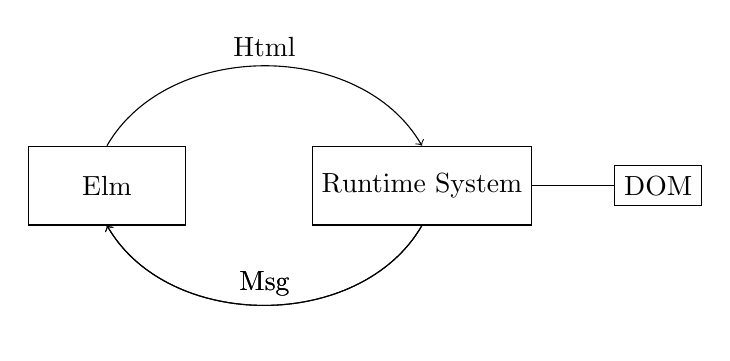
\begin{tikzpicture}
  % Nodes
  \node (p) [rectangle, draw, minimum height=1cm, minimum width=2cm] at (0, 0) {Elm};
  \node (i) [rectangle, draw, minimum height=1cm, minimum width=2cm] at (4, 0) {Runtime System};
  \node (d) [rectangle, draw, minimum height=0.5cm, minimum width=1cm] at (7, 0) {DOM};
  % Arrow
  \draw[->] (p.north) to[out=60, in=120] node[midway, above] {Html} (i.north);
  \draw[->] (i.south) to[out=-120, in=-60] node[midway, above] {Msg} (p.south);
  \draw[->] (i.south) to[out=-120, in=-60] node[midway, above] {Msg} (p.south);
  \draw[] (i) -- (d) node[midway, above] {};
  % Header
\end{tikzpicture}

  \caption{Elm Architecture (Figure adapted from \cite{elmFig})}
  \label{fig:elmArchitecture}
\end{figure}

\subsection{Module Architecture}

In this application, the Elm-box is a module, while the runtime system, is the
core itself. The core invokes all modules, all of which, should have these three
functions, \lstinline{init}, \lstinline{update}, and \lstinline{view}.

\paragraph{Init} Returns a collection of key-value-pairs, which represent
the state of the core.

\paragraph{Update} Returns a collection of key-value-pairs, which
overwrite existing key-value-pairs in the state, or are appended to the state.
Invoked every time a \textit{Msg} is sent.

\paragraph{View} Returns a collection which represents \gls{html},
which is rendered by the core.

\begin{center}
  \lstinputlisting
    [ language=Haskell
    , caption={Module Type}
    , label=lst:pluginExample
    ]{./code/plugin-example.hs}
\end{center}

A module is initialized by invoking the \textbf{init} method, which returns a
state. This can be seen in figure \ref{fig:moduleInit}. After the state
initialization, the modules' \textbf{view} method is invoked, which initializes
the \gls{ui} for the user, which can be seen in figure \ref{fig:moduleInitView}.

\begin{figure}
  \centering
  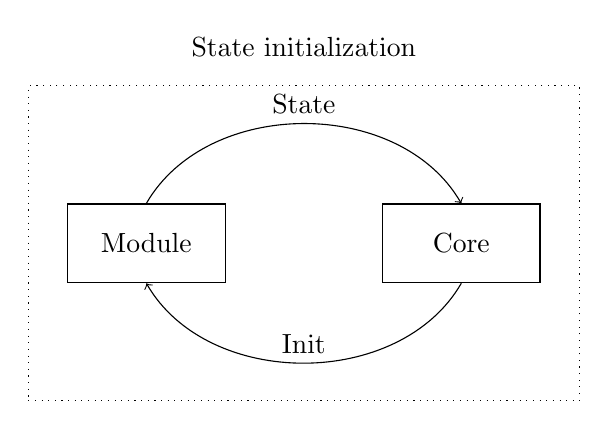
\begin{tikzpicture}
  \node [rectangle, draw, minimum height=4cm, minimum width=7cm, dotted] at (2, 0) {};
  \node [] at (2, 2.5) {State initialization};

  \node (i) [rectangle, draw, minimum height=1cm, minimum width=2cm] at (4, 0) {Core};
  \node (p) [rectangle, draw, minimum height=1cm, minimum width=2cm] at (0, 0) {Module};
  \draw[->] (p.north) to[out=60, in=120] node[midway, above] {State} (i.north);
  \draw[->] (i.south) to[out=-120, in=-60] node[midway, above] {Init} (p.south);
\end{tikzpicture}

  \caption{Module state initialization stage}
  \label{fig:moduleInit}
\end{figure}

\begin{figure}
  \centering
  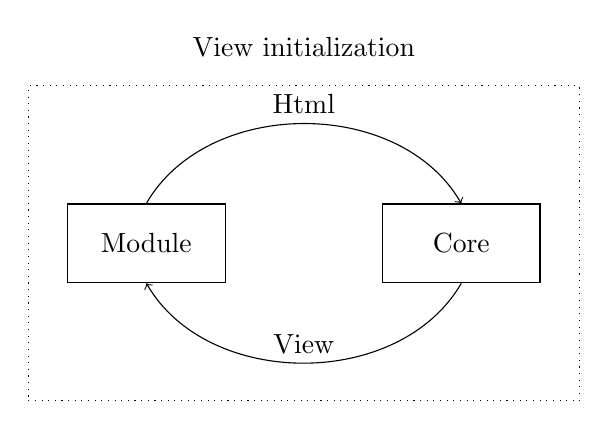
\begin{tikzpicture}
  \node [rectangle, draw, minimum height=4cm, minimum width=7cm, dotted] at (2, 0) {};
  \node [] at (2, 2.5) {View initialization};

  \node (i) [rectangle, draw, minimum height=1cm, minimum width=2cm] at (4, 0) {Core};
  \node (p) [rectangle, draw, minimum height=1cm, minimum width=2cm] at (0, 0) {Module};
  \draw[->] (p.north) to[out=60, in=120] node[midway, above] {Html} (i.north);
  \draw[->] (i.south) to[out=-120, in=-60] node[midway, above] {View} (p.south);
\end{tikzpicture}

  \caption{Module view initialization stage}
  \label{fig:moduleInitView}
\end{figure}

\todo{Explain the module architecture in IDE terms, so with IDE examples}

Since the \gls{ide} is written in both TypeScript and Rust, a method of encoding
type information when crossing between the TypeScript and Rust environment was
needed. It was achieved by simply typing \gls{json} objects, so while the state
could be represented as any \gls{json} object, it was instead represented as
nested \gls{json} objects, where, all values, except \textbf{null}, where
encoded as an object with one field, being the type of the object, and then the
value. So an int would be \textbf{\{ int: 0 \}}.

The reason for representing a JSON object as key-value pairs, is that this could
be easily translated to a Rust representation of the same type, using the
\textit{Serde} crate. This allows for creating Rust structs which represents
JSON objects, and creates an automatic encoder/decoder between Rust and JSON.
This ensures a good cooperation between the \textit{frontend} and
\textit{backend}.
\todo{Rewrite}

The general idea was that for each possible \gls{dom}-event, there would exist a
way to send a Msg. Each Msg contains a Msg name, and some value, which enabled
pattern matching on Msg, similar to Elm, for modules, so each module could
choose to act on a Msg or not.

In listing \ref{lst:pluginCounterExample}, an example of a counter module can be
seen. This module initializes a state, containing the field \textbf{"counter"},
with the value \textbf{VInt 0}.

The \textit{update} function the module exposes, matches on a \textbf{"counter"}
msg, with a \textbf{VInt i} value. If the given Msg matches this, then the
module adds to the \textbf{"counter"}-field, the value from the Msg, which is
$1$.

Finally, the \textit{view} function renders a button, which when pushed by a
user, sends the \textit{counter-Msg}.

\begin{center}
  \lstinputlisting
    [ language=Haskell
    , caption={Module Architecture}
    , label=lst:pluginCounterExample]{./code/plugin-counter-example.hs}
\end{center}

\subsubsection{Module purity}

One important thing in this architecture, is the pureness of module. The state
of a module needs to be kept in the core application, and not in the module
itself. The reason for this is twofold. It allows for the possibility of the
core to be optimized in the future, as modules which do not react to a certain
msg-state combination, can be noticed, and ensure modules are not unnecessarily
invoked. It also lowers the complexity for module developers, as it is easier to
reason about modules if \textit{all} they do is read or write to some state.

If we have the modules $A$ and $B$, where their relationship is $A \to B$,
meaning $A$ \textit{invokes} $B$ by sending some Msg, which $B$ reacts too, and
we want something to happen before $B$ reacts, we can add a new module, $C$,
which also reacts to the same Msg, but if we know the name of the module $B$,
we can set the name of module $C$ to be \textit{above} the order, relative to
$B$, ensuring that $C$ always triggers before $B$.

But this introduces a possibility for some hierarchy in the module ecosystem.
For example, a module could act as a framework, and therefore needs to only be
loaded once, creating new locations, with styling.

\subsection{Module v2 Cons}

\subsubsection{Module v2 cons}

\todo{Sum up all the issues with this architecture}

\begin{enumerate}
  \item React sucks
  \item Modules cannot invoke modules
  \item Slow
  \item Not asynchronous
  \item Ever growing state
\end{enumerate}


With this setup, however, the state is appending/overwriting -only, which means
the state can only grow.

This setup is also not really modular, as a single module cannot invoke another
module without being impure. The only way to invoke/trigger another module, is
to throw a \textit{Msg}, which would trigger an update -> view -> cycle. So
a module cannot \textit{listen} for a single message, all modules are triggered
by the same \textit{Msg}, and handled accordingly.

\subsubsection{State Collision} \label{sec:collision}

A state collision occurs when two or more modules updates the same field, during
the same update-cycle. This issue also occurs when folding two states.

Was \textit{solved} with this:

\begin{center}
  \lstinputlisting
  [ language=Haskell
  , caption={State Collision Typing}
  , label=lst:stColType
  ]{./code/state-collision-types.hs}
\end{center}

Takes list of states from all modules, checks for collisions. It returns a
list of
\lstinline[language=Haskell]{Either [(String, State)] ([(String, State)], String)}.
If it is a collision, then it's a
\lstinline[language=Haskell]{Right ([(String, State)], String)}, which is a
tuple where the first element is a list of tuples, being the module and their
state, and the last element being the field that the collision occurred on.
The other value: \lstinline[language=Haskell]{Left [(String, State)]}, are the
module state that has no collision.

\paragraph{Collision} A collision between two states occurs if they share the same
field.

There are several different ways to correct a collision between two
states:

\begin{enumerate}
  \item If the states are of same type:
    \begin{enumerate}
      \item If the value from one of the colliders are unchanged from the previous state:
        \begin{enumerate}
          \item Keep the new value OR Keep the old value
        \end{enumerate}
      \item Else
        \begin{enumerate}
          \item Apply the types' semigroup operator to the fields.
        \end{enumerate}
    \end{enumerate}
  \item Else
    \begin{enumerate}
      \item If the value from one of the colliders are unchanged from the previous state:
        \begin{enumerate}
          \item Keep the new value OR Keep the old value
        \end{enumerate}
      \item Else
        \begin{enumerate}
          \item Keep the left-hand side value OR Keep the right-hand side value
        \end{enumerate}
    \end{enumerate}
\end{enumerate}

Since the states are ordered by the name of the module they come from, we
have a consistent ordering of left-hand side and right-hand side. If the same
modules give a collision on the same input, (given that all modules are pure), the
resulting state will be the same every time. The problem is that applying some
function on the values could be an unwanted way to resolve collisions. The
standard way will be to log the collision, and then drop both states. Even
if two states have A and B amount of fields, and just one collision, we will
drop A + B amount of fields. Therefore, a module developer should avoid
collisions.

\begin{center}
  \lstinputlisting
  [ language=Haskell
  , caption={State Collision}
  , label=Listing
  ]{./code/state-collision.hs}
\end{center}

\todo{Mention how updating two fields on the same object also counts as a collision}

This problem of resolving state collision only occurs because each module
returns a subtree of the state. We then have to analyze the new coalesced tree
for each new subtree that is added, to figure out if there occurs any collision.
And then notifying the module developer of which field this collision occurred
on, and which modules tried to modify that field.

\section{Module V.3} \label{sec:mod3}

The third and hopefully final, plan:

\begin{enumerate}
  \item Everything is a module
  \item Modules can \textit{invoke} modules
\end{enumerate}

A module only exposes two functions:

\paragraph{Init} Returns nothing

\paragraph{Handler} Returns nothing

In the previous architecture version, each module directly changed the state,
which caused issues. Instead, each modification a module does, \textit{acts}, as
a direct modification, but is in fact, translated to a DSL which can be analyzed
for possible collisions. This was discovered to be a need, as in the new
version, the \gls{ui} was also restructured, to allow for less re-rendering, and
this restructuring, made it clear that changing the state, or changing the
\gls{ui} is just tree manipulations, which will be discussed more later.

\subsection{Zero core architecture and microservice architecture}

The new plan came with a change of viewpoint. Think of
\textit{everything being a module}, this pushed for a modularization between the
then tightly coupled parts, the \textit{frontend} and \textit{backend}. As
mentioned, having two different languages could allow for easier support of
modules written in different programming languages, but for this to work in an
optimal way, both the \textit{frontend} and \textit{backend} should be loosely
coupled. This is an equivalent architecture to microservices.
\todo{Add diagrams and examples}
\todo{Mention runtimes}

\subsection{Vanilla TypeScript}

Instead of using React as the frontend framework, TypeScript was chosen, which
simplified the integration between the backend and frontend, as the complexity
of React's state management could be avoided, along with React's hydration.
Given the rendering was now more \textit{hands-on}, the core could expose a lot
of the functionality for rendering, which modules could change. This would
increase the difference between the \gls{jsms} and \gls{rsms}, as the backend
was not privy to this API, but this was not seen as an issue, as this API would
turn module non-pure.
\todo{Mention pureness earlier}

\subsubsection{Removing abstractions}

It became prudent, due to the change of architecture, to change the entire
frontend, moving away from React, and using \textit{bare-bones} TypeScript. This
would enable easier integration into the \gls{jsms}.

\subsection{Core Modifications}

Learning from the issues outlined in section \ref{sec:collision}, instead of a
module returning the new core, it will rather return a set of instruction on
\textit{how} the core is to be modified, resulting in what the module developer
wants the core to be. The reason for turning it around in this manner, is that,
the new architectural change also came with a change on how the \gls{ui} is
modeled, as it is now up to the core to figure out an inexpensive way to do
rendering. Since the core has \gls{ui}-structure which is a representation of
what the \gls{dom} should be, it can be treated as a Virtual-\gls{dom}, similar
as to how React does it. This also means that there could be a collision on
\gls{ui}-change, as well as on a state-change. Instead of solving the equivalent
problems twice, it was decided to try to treat the issues with collisions in
state and \gls{ui} as the same issue; its some form of tree-manipulation.

\begin{center}
  \lstinputlisting
    [ language=Haskell
    , caption={Core}
    , label=lst:coreAdt
    ]{./code/module-example-core.hs}
\end{center}

In listing \ref{lst:moduleEvent}, one can see the structure of an
\lstinline[language=Haskell]{Event}. This allows for modules to
pattern match on specific \lstinline[language=Haskell]{Event}s, and as in the
previous version, only react to specific \lstinline[language=Haskell]{Event}s.
What is different, is as shown in the \ref{lst:moduleCounter} listing, is that
each module registers an \lstinline[language=Haskell]{EventHandler} which is
\textit{only} invoked when the specific \lstinline[language=Haskell]{Event} it
is registered with, is called. This ensures a more direct form of
module-to-module communication, as a module can directly \textit{invoke} another
module. This changes the structure of the module architecture to go from one
wherein the core is a terminal object, to a more \textit{complicated} one, in
which module families can form.

\begin{center}
  \lstinputlisting
    [ language=Haskell
    , caption={Module Event Type}
    , label=lst:moduleEvent
    ]{./code/module-example-event.hs}
\end{center}

\begin{center}
  \lstinputlisting
    [ language=Haskell
    , caption={Module Counter Example}
    , label=lst:moduleCounter
    ]{./code/module-example-counter.hs}
\end{center}

\begin{center}
  \lstinputlisting
    [ language=Haskell
    , caption={Module Counter Example Event Handler}
    , label=lst:moduleEventHandler
    ]{./code/module-example-counter-handler.hs}
\end{center}

The module example shown in listing \ref{lst:moduleCounter} and
\ref{lst:moduleEventHandler}, is again, a simple counter example, where the
module registers a \lstinline[language=Haskell]{CoreModification}, changing the
UI-hierarchy, by adding a button which throws an
\lstinline[language=Haskell]{Event} that is handled by the
\lstinline[language=Haskell]{EventHandler} shown in
\ref{lst:moduleEventHandler}, which again, modifies the core by changing the
counter field with the value from the \lstinline[language=Haskell]{Event}.

\subsection{Tree Manipulation}

\todo{
  Mention Magnolia here, and how the satisfaction/unit test thing can "prove"
  this
}
This restructure changes the way the view is rendered. Instead of the view being
re-rendered for each state-update, the view, or \gls{ui}-hierarchy, is only
\todo{Mention earlier how React was used/considered due to the "smart" re-rendering}
modified by modules. This modification is similar to the earlier state
modification, so a unified algorithm to solve this can be used. If there is an
easy way to translate a \gls{ui} modification to a state modification, and back
again. To solve this, instead of having a module return the actual
modifications, meaning, the updated core, a module returns a set of instructions
of what to do with the core.

\begin{center}
  \lstinputlisting
   [ language=Rust
   , caption={Instruction (Rust)}
   , label=lst:inst
   ]{./core/src-tauri/core-std-lib/src/instruction.rs}
\end{center}

The listing \ref{lst:inst}, shows of how the \textbf{Instruction}-set makes the
modification of the core, a kind of group, as given the definition
\ref{def:group}, we can construct one:

\begin{theorem}[Instruction Group]
  Let $\Sigma$ be the set of all strings, $Val$ be the set of all
  \textbf{Values}, $Html$ be the set of all \textbf{Html} variants, and
  $Inst_{val}$ be the set of all \textbf{Instruction} defined as:
  $$
    NoOp = \left \{ noOp \right \}
  $$
  $$
    NoOp \in Inst_{val}
  $$
  $$
    Add_{val} = \left \{ (x, y, z) \vert x \in \Sigma, y \in \Sigma, z \in Val \right \}
  $$
  $$
    Add_{val} \in Inst_{val}
  $$
  $$
    Rem_{val} = \left \{ (x, y, z) \vert x \in \Sigma, y \in \Sigma, z \in Val \right \}
  $$
  $$
    Rem_{val} \in Inst_{val}
  $$
  $$
    Then_{val} = \left \{ (x, y) \vert x, y \in Inst_{val} \right \}
  $$
  $$
    Then_{val} \in Inst_{val}
  $$
  For any $x \in Add_{val}$ there exist a unique $y \in Rem_{val}$, such that:
  $$
    x \oplus y = noOp
  $$
\end{theorem}

This, unfortunately, cannot be encoded in Rusts type system, but when implementing
$combine$, we can map the variants along with the specific fields being added
($Add$), modified ($Mod$), or removed ($Rem$), to get a more optimized
instruction set. If we are modifying a value on field $foobar$, but in the same
instruction set, remove it, then the modifying instruction is an $NoOp$.

\todo{Add trivial module example, or something}

Using this as a module developer is quite abstract, so to facilitate development
of modules, a helper class was created, which \textit{translates} modifications
to instructions. As shown in listing \ref{lst:ui-builder} and
\ref{lst:state-builder}, a module developer simply invokes different methods on
the builder, eventually building a \textbf{CoreModification}, to be sent.

\begin{center}
  \lstinputlisting
   [ language=Rust
   , caption={UI Builder (Rust)}
   , label=lst:ui-builder
   ]{./code/module-ui-builder.rs}
\end{center}

\begin{center}
  \lstinputlisting
   [ language=Rust
   , caption={State Builder (Rust)}
   , label=lst:state-builder
   ]{./code/module-state-builder.rs}
\end{center}

This allows for an ergonomic way for module developer to create modifications on
the core, without having to understand the syntax of the
\textbf{Instruction}-set.

\begin{center}
  \lstinputlisting
   [ language=Haskell
   , caption={Module Type}
   , label=lst:moduleType
   ]{./code/module-example.hs}
\end{center}

As one can see in listing \ref{lst:moduleType}, a module only exposes its name,
and an \lstinline[language=haskell]{init} function, which takes the
\lstinline[language=haskell]{Core}, which is a representation of
the core application shown in listing \ref{lst:coreAdt}.

\subsection{Backend Agnostic Frontend}
\todo{This is not true anymore}

As mentioned in the previous section, the tech stack splits the application into
two, loosely coupled parts. The \textit{frontend} and \textit{backend}. This
architecture does facilitate the concept of an agnostic frontend. That is, if,
as is the case per the previous plan, all logic pertaining to the core is in the
\textit{frontend}, cannot the backend be anything, as long as it fulfills the
following criteria.

\subsection{Making the Core evaluate modifications asynchronously}

Due to Rust first class focus on concurrency, it was trivial to make the core
modifications run asynchronously. In previous iterations, the core evaluated
one event at a time, waiting until all modules had finished their computations,
before emulating the change and allowing for the next event to be evaluated. But
this caused a noticeable \textit{lag} if an event was long. This was solved by
changing the core modification evaluation from a simple method to be invoked, to
an \gls{mpsc} channel system. Using \textit{tokio}, a Rust crate for
asynchronous development, a channel for core modifications was created, and
instead of the core collecting all modifications, each module is invoked and
\textit{awaited} for in a separate thread, where in each module, if they have a
core modification, sends the modification to the core channel, which works on
a first come, first server basis. Here the core can evaluate the changes, also
on a separate thread.
\todo{Mention in v2 how file system stuff made stuff sluggish}

\begin{itemize}
  \item File system modification
  \item Module loading
\end{itemize}

\section{Testing} \label{sec:testing}

\todo{Showcase example of testing the ide}

A zero-core application is equivalent to a microservice architecture, in that
testing is important to ensure changes in one module does not inadvertently
affect another.

\subsection{Mocking}

Due to the \textit{pureness} of modules, mocking can be achieved easily, and
therefore, modules can be tested alone, which is good, because testing a
singular module is inexpensive.

\subsection{Unit Testing}

A module developer should create unit tests for their module. This can easily be
done, and tested many times, due to the light-weightiness of a module.

\subsubsection{UI Testing}

\todo{Mention of ui testing is part of unit testing}

\subsection{Module Family Testing}

If a module changes some feature, let's say in the editor functionality, the
module family tree encompassing this functionality needs to be tested, to ensure
nothing breaks.

\subsubsection{Contract Testing}

As a module developer, on is designing some kind of \gls{api}, but the developer
has no say in how a consumer of the \gls{api} consumes it. In a microservice
architecture, the common way to work around this, is to version control the
\gls{api} by prefixing \textit{v*} in front of all endpoints in the \gls{api},
where star, (*), is the version of the \gls{api}. This way, the \gls{api}
designer can develop new \gls{api}s, without worrying about breaking
functionality that consumers of the \gls{api} depend on. This, however, usually
means having to maintain equivalent \gls{api}s in parallel, until one decides
to deprecate an older less used version, forcing consumers to move on to the
newer version of the \gls{api}.

Instead of relying on such a versioning system, module developers could use
\textit{contract testing}.

\paragraph{Contract Testing} Imagine some \gls{api}, and several consumers,
$A, B, C$, The \gls{api} developer is serving some data, in this case an
integer number, which all the consumers use. One day, the developer finds out
that using integers is not optimal, and want to move on to using floating point
numbers instead. Changing the \gls{api} outright could bring issues, as the
consumers might rely on the \gls{api} being an integer, instead of a float. But
the change is needed, or wanted, at least. In this scenario, it is \textit{easy}
to inform all the consumers of the \gls{api}, but if the consumer count
increases tenfold, this is more difficult. A notice can still be sent, but it is
not feasible to ensure all consumers commit time to change their ways. Contract
testing ensures that, if a change like this occurs, the maintainer of the
\gls{api} is notified by which consumer this change breaks.

The issue is to create these contracts. Using frameworks like Pact \cite{pact},
a developer creates a \gls{dsl} test, where they describe how the provider or
consumer reacts to certain interactions. But since everything is a module, we
can automate this.

\subsection{Automating Contract Testing}

This process could be partially automated, as all modules have to register the
event they want to handle. Furthermore, all events thrown are also explicitly
done through the core instance, meaning a \textit{test-core} could be created,
which registers which event is thrown from what module, and all dependencies
between modules can be noted.
\todo{Implement this}

\subsection{End-To-End-Testing}

The final step in the testing pipeline, is to test the entire application
together. This is known as \gls{e2e}, but this is expensive.

\section{Modules}

\todo{Introduction}

Here are some examples of modules implemented using the proposed architecture.

\subsection{Magnolia Dependency Graph Visualizer}

\todo{Implement and showcase this module}

\subsection{IDE Module Family}

\todo{Showcase the modules created to have a rudimentary IDE}
\todo{Mention QOF modules for future module developers}
\todo{Mention Project Management}

\subsection{Caching}
\todo{Properly implement this}
In Magnolia, caching of \gls{lsp} queries is important. And caching of the
compiled code.

\subsection{Editor Module Family}

\todo{Implement a rudimentary editor}

\subsection{Magnolia Language Server}

\todo{Implement a rudimentary Magnolia LS}
